\documentclass{ximera}

\title{Optimization Review}
\author{Zack Reed}

\begin{document}
\begin{abstract}
In this activity we review single-variable optimization, which we will then extend in the next sections to multivariable settings.
\end{abstract}
\maketitle

\section*{Introduction: Why Optimize?}

Optimization is everywhere in modern applications:
\begin{itemize}
    \item Machine learning models minimize error functions
    \item Engineers maximize efficiency while minimizing cost
    \item Physicists find states of minimum energy
    \item Economists maximize profit while minimizing waste
\end{itemize}

In single-variable calculus, we found extrema by setting $f'(x)=0$ and testing with the second derivative. In multivariable settings, we need new tools!

\begin{problem}
Review: In single-variable calculus, to find the minimum of $f(x) = x^2 - 4x + 5$, we would:

\begin{enumerate}
    \item Find the critical point by solving $f'(x) = \answer{2x-4} = 0$, giving $x = \answer{2}$.
    \item Check the second derivative: $f''(x) = \answer{2}$.
    \item Since $f''(2) > 0$, we conclude this is a \wordChoice{\choice{maximum}\choice[correct]{minimum}\choice{saddle point}}.
    \item The minimum value is $f(2) = \answer{1}$.
\end{enumerate}

\begin{feedback}
    This process extends to multivariable functions, but with new twists! We'll need gradients instead of derivatives, and the Hessian matrix instead of the second derivative.
\end{feedback}
\end{problem}

Before digging into the weeds of multivariable techniques, let's review why we use these first and second derivatives in the first place.

\begin{problem}
Explore the following applet to see how the first derivative tests works.

This applet begins by assuming that we have found \textbf{critical points} at $x=-4$, $x=4$, and $x=10$. This means that we've already computed $f'(x)$, and have verified that $f^\prime(-4)=0$, $f^\prime(4)=0$, and $f^\prime(10)=0$. 

This is where most students make the mistake of stopping their analysis. Just because the derivative is zero at these points does not guarantee that they are maxima or minima!

\begin{expandable}{stuff}{GeoGebra Instructions}
    Read the text on screen and advance the animation by clicking the buttons (in red or black text) to view new text, tangent lines, and portions of the graph. Use the reset button at the bottom left to start over.
\end{expandable}
\begin{center}
\geogebra{ebuvppdr}{757}{611}
\end{center}

After exploring the applet, identify what you observed (Select All that are true):
\begin{selectAll}
    \choice[correct]{When $f'(x) > 0$, the graph is increasing}
    \choice[correct]{When $f'(x) < 0$, the graph is decreasing}
    \choice{When $f'(x) = 0$, the graph is always a maximum or minimum}
    \choice{The first derivative measures the concavity of the function}
    \choice[correct]{At points where $f'(x) = 0$, there may be a local maximum or minimum, but further testing is needed.}
\end{selectAll}

\begin{feedback}
The first derivative measures the function's rates of change, telling us when it increases and decreases. If the derivative is zero, there is possible a local max or min, but you need to test around the point to be sure.
\end{feedback}
\end{problem}

The first derivative tells us where the functions have \textbf{possible} maximum and minimum values. We can also use the first derivative directly to verify whether we actually have maxima or minima.

When we move to higher dimensions, the 2nd derivative is easier to use in traditional optimization. The first derivative is instead used for something called \emph{gradient descent}, which we will discuss in a few sections.

\begin{problem}
Let's review how we use the second derivative to tell us about critical the critical points of a function.

\begin{expandable}{stuff}{GeoGebra Instructions}
    Read the text on screen and advance the animation by clicking the buttons (in red or black text) to view new text, tangent lines, and portions of the graph. Use the reset button at the bottom left to start over.
\end{expandable}

\begin{center}
\geogebra{uervaqau}{757}{611}
\end{center}

After exploring the applet, identify what you observed (Select All that are true):
\begin{selectAll}
    \choice[correct]{When $f''(x)  > 0$, the graph bends upward}
    \choice[correct]{When $f''(x) < 0$, the graph bends downward}
    \choice{When $f''(x) = 0$, the graph is always a straight line}
    \choice{The second derivative measures the slope of the function}
\end{selectAll}

\begin{feedback}
The second derivative measures how the first derivative (slope) changes, not the slope itself. This rate of change of slope is what we call concavity.
\end{feedback}
\end{problem}


\section*{Caution: Not All Critical Points are Extrema!}

In single-variable calculus, we weren't always guaranteed a max or min at critical points. The same is true in multivariable calculus.

\begin{problem}
Let's first review this issue with the function $f(x) = x^3$.

\begin{center}
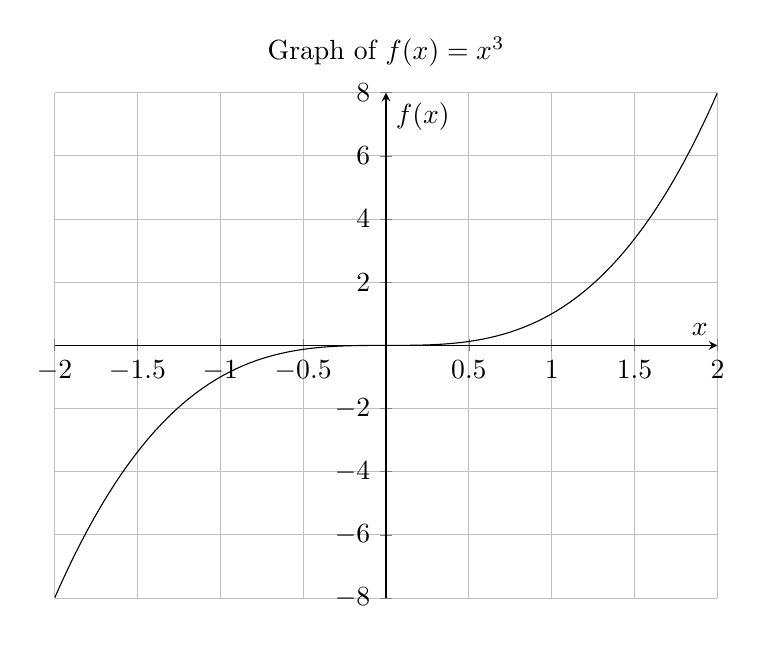
\begin{tikzpicture}
    \begin{axis}[
        axis lines = center,
        xlabel = $x$,
        ylabel = {$f(x)$},
        title = {Graph of $f(x) = x^3$},
        width=10cm,
        height=8cm,
        grid=major,
    ]
    \addplot[domain=-2:2,samples=100] {x ^3};
    \end{axis}
\end{tikzpicture}
\end{center}

Even though the derivative is zero at $x=0$, if you move forward in $x$, the function \wordChoice{\choice{decreases}\choice[correct]{increases}}; and if you move backward in $x$, the function \wordChoice{\choice{decreases}\choice[correct]{increases}}. So there \wordChoice{\choice[correct]{is no}\choice{is a}} max or min at this critical point!
\end{problem}



\end{document}
